\documentclass[]{article}
\usepackage{lmodern}
\usepackage{amssymb,amsmath}
\usepackage{ifxetex,ifluatex}
\usepackage{fixltx2e} % provides \textsubscript
\ifnum 0\ifxetex 1\fi\ifluatex 1\fi=0 % if pdftex
  \usepackage[T1]{fontenc}
  \usepackage[utf8]{inputenc}
\else % if luatex or xelatex
  \ifxetex
    \usepackage{mathspec}
  \else
    \usepackage{fontspec}
  \fi
  \defaultfontfeatures{Ligatures=TeX,Scale=MatchLowercase}
\fi
% use upquote if available, for straight quotes in verbatim environments
\IfFileExists{upquote.sty}{\usepackage{upquote}}{}
% use microtype if available
\IfFileExists{microtype.sty}{%
\usepackage{microtype}
\UseMicrotypeSet[protrusion]{basicmath} % disable protrusion for tt fonts
}{}
\usepackage[margin=1in]{geometry}
\usepackage{hyperref}
\hypersetup{unicode=true,
            pdftitle={DATA 609 - Homework 3},
            pdfauthor={Joshua Sturm},
            pdfborder={0 0 0},
            breaklinks=true}
\urlstyle{same}  % don't use monospace font for urls
\usepackage{graphicx,grffile}
\makeatletter
\def\maxwidth{\ifdim\Gin@nat@width>\linewidth\linewidth\else\Gin@nat@width\fi}
\def\maxheight{\ifdim\Gin@nat@height>\textheight\textheight\else\Gin@nat@height\fi}
\makeatother
% Scale images if necessary, so that they will not overflow the page
% margins by default, and it is still possible to overwrite the defaults
% using explicit options in \includegraphics[width, height, ...]{}
\setkeys{Gin}{width=\maxwidth,height=\maxheight,keepaspectratio}
\IfFileExists{parskip.sty}{%
\usepackage{parskip}
}{% else
\setlength{\parindent}{0pt}
\setlength{\parskip}{6pt plus 2pt minus 1pt}
}
\setlength{\emergencystretch}{3em}  % prevent overfull lines
\providecommand{\tightlist}{%
  \setlength{\itemsep}{0pt}\setlength{\parskip}{0pt}}
\setcounter{secnumdepth}{0}
% Redefines (sub)paragraphs to behave more like sections
\ifx\paragraph\undefined\else
\let\oldparagraph\paragraph
\renewcommand{\paragraph}[1]{\oldparagraph{#1}\mbox{}}
\fi
\ifx\subparagraph\undefined\else
\let\oldsubparagraph\subparagraph
\renewcommand{\subparagraph}[1]{\oldsubparagraph{#1}\mbox{}}
\fi

%%% Use protect on footnotes to avoid problems with footnotes in titles
\let\rmarkdownfootnote\footnote%
\def\footnote{\protect\rmarkdownfootnote}

%%% Change title format to be more compact
\usepackage{titling}

% Create subtitle command for use in maketitle
\newcommand{\subtitle}[1]{
  \posttitle{
    \begin{center}\large#1\end{center}
    }
}

\setlength{\droptitle}{-2em}

  \title{DATA 609 - Homework 3}
    \pretitle{\vspace{\droptitle}\centering\huge}
  \posttitle{\par}
    \author{Joshua Sturm}
    \preauthor{\centering\large\emph}
  \postauthor{\par}
      \predate{\centering\large\emph}
  \postdate{\par}
    \date{September 28, 2018}


\begin{document}
\maketitle

\hypertarget{chapter-3-problems}{%
\section{Chapter 3 Problems}\label{chapter-3-problems}}

\hypertarget{page-113-exercise-2}{%
\subsection{1 (Page 113, exercise \#2)}\label{page-113-exercise-2}}

The following table gives the elongation \(e\) in inches per inch
(in./in.) for a given stress \(S\) on a steel wire measured in pounds
per square inch (lb/in\(^2\)). Test the model \(e = c_1S\) by plotting
the data. Estimate \(c_1\) graphically.

\begin{verbatim}
##   [,1] [,2] [,3] [,4] [,5] [,6] [,7] [,8] [,9] [,10] [,11]
## S    5   10   20   30   40   50   60   70   80    90   100
## e    0   19   57   94  134  173  216  256  297   343   390
\end{verbatim}

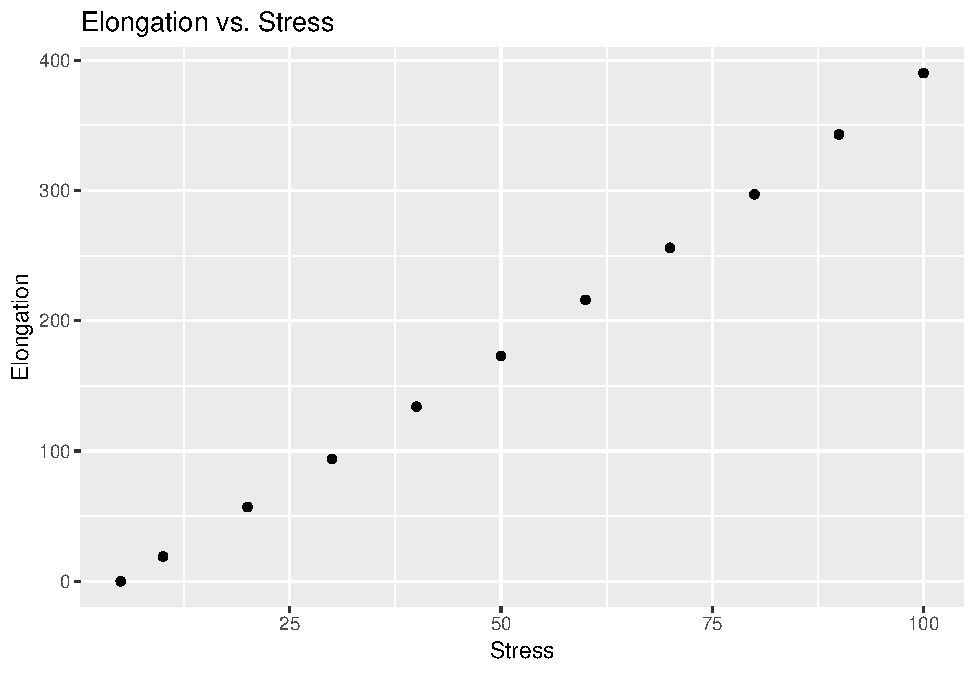
\includegraphics{Joshua_Sturm_Homework3_files/figure-latex/unnamed-chunk-1-1.pdf}

We can estimate the slope using the first and 6th points.

\begin{equation*}
c_1 = \frac{173 - 0}{50 - 0} = 3.46
\end{equation*}

\hypertarget{page-121-exercise-2.a}{%
\subsection{2 (Page 121, exercise \#2.a)}\label{page-121-exercise-2.a}}

Formulate the mathematical model that minimizes the largest deviation
between the data and the line \(y = ax + b\). If a computer is
available, solve for the estimates of \(a\) and \(b\).

\begin{verbatim}
##   [,1] [,2] [,3] [,4] [,5] [,6]
## x  1.0  2.3  3.7  4.2  6.1  7.0
## y  3.6  3.0  3.2  5.1  5.3  6.8
\end{verbatim}

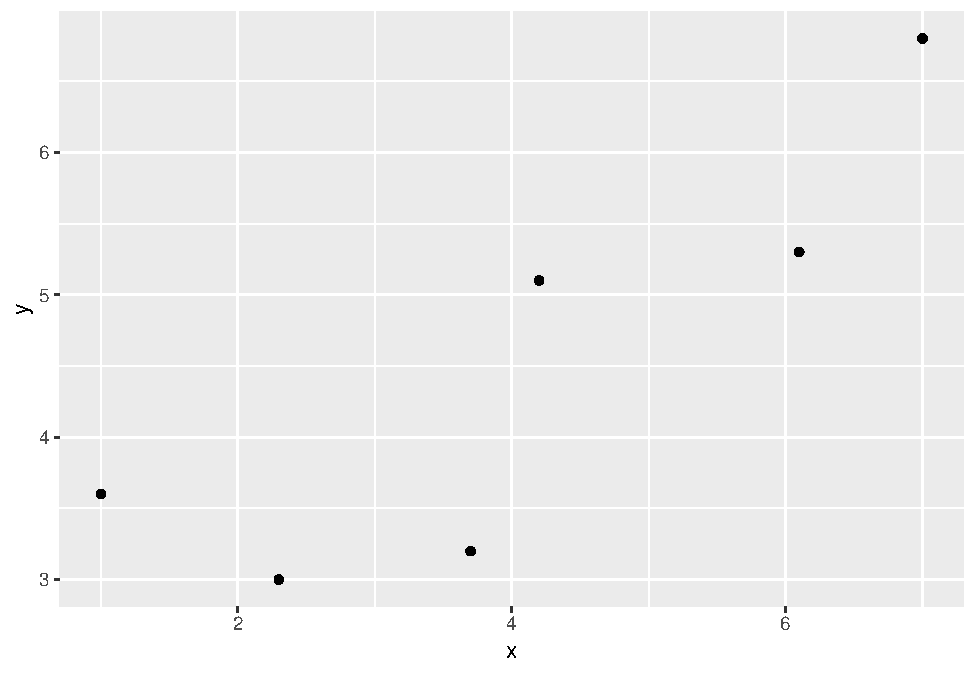
\includegraphics{Joshua_Sturm_Homework3_files/figure-latex/unnamed-chunk-2-1.pdf}

We can fit a model using these data points to minimize the deviation.

\begin{verbatim}
## 
## Call:
## lm(formula = y ~ x, data = devdf)
## 
## Residuals:
##       1       2       3       4       5       6 
##  0.8209 -0.5126 -1.1025  0.5154 -0.3567  0.6355 
## 
## Coefficients:
##             Estimate Std. Error t value Pr(>|t|)  
## (Intercept)   2.2149     0.7737   2.863   0.0458 *
## x             0.5642     0.1703   3.313   0.0296 *
## ---
## Signif. codes:  0 '***' 0.001 '**' 0.01 '*' 0.05 '.' 0.1 ' ' 1
## 
## Residual standard error: 0.8586 on 4 degrees of freedom
## Multiple R-squared:  0.7329, Adjusted R-squared:  0.6661 
## F-statistic: 10.98 on 1 and 4 DF,  p-value: 0.02957
\end{verbatim}

The largest deviation is 1.1025182.

The equation for the line of best fit is \begin{equation*}
y = 0.5642337x + 2.2148534
\end{equation*}

Viewing the fitted model:

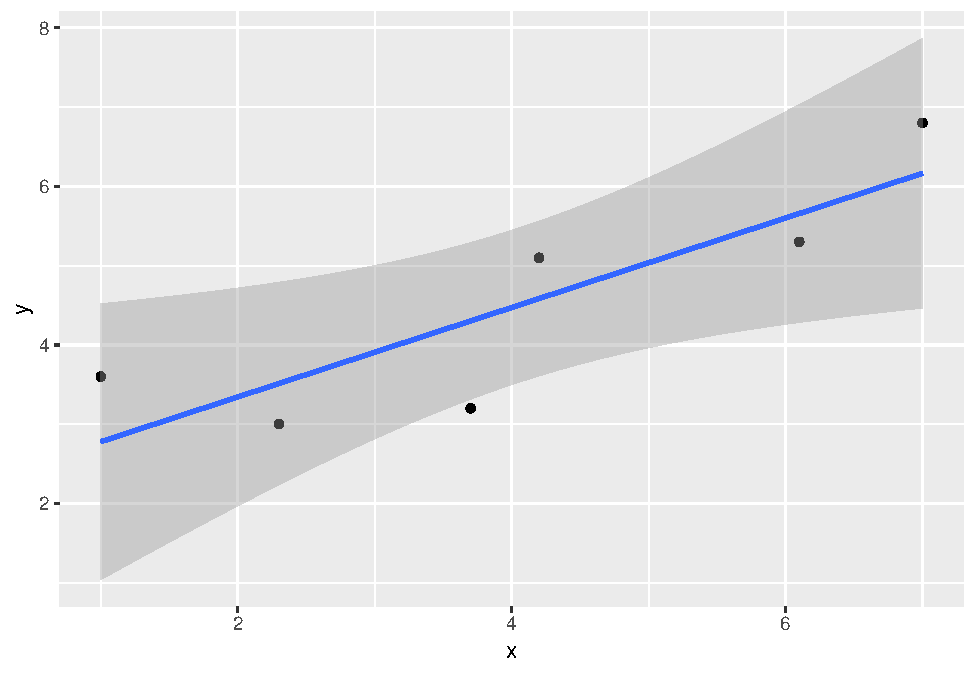
\includegraphics{Joshua_Sturm_Homework3_files/figure-latex/unnamed-chunk-4-1.pdf}


\end{document}
